%--------------------------------------------
%    Introduction
%--------------------------------------------
\section{Introduction}

Digital image can degraded by noise in the process of capture, acquisition, processing and transmission. Therefore, image denoising is one of the fundamental challenges in the field of image processing and computer vision with the objective to eliminate the noise from given noisy image in data acquisition to predict original image. A good image denoising model is eliminating noise as much as possible while preserving the characteristics of the image such as edges, corners and other sharp structures, etc.\cite{Motwani2004}

Two main approach to image denoising is based on spatial domain, and transform domain. Besides, there are some image denoising methods implemented in both spatial and transform domain.

Approaching denoise in spatial domain, Tomasi et. al \cite{Tomasi1998} proposed a new a nonlinear, edge preserving and noise-reducing smoothing filter for images called Bilateral Filter. Bilateral filter \cite{Paris2008} solves the limitation of Gaussian filter \cite{Gonzalez06DIP} by taking in account the difference in value with the neighborhood to preserve edges while smoothing.  In bilateral filter, the influence of a pixel to another one should not only occupy a nearby location but also have a similar value. Though bilateral may not be the best noise reducing filter but it is good and simple. Also, it can be used for tone mapping, relighting and texture editing. However, the nonlinear operator is hard to compute since it is complex and spatially varying kernels. Besides, it causes staircase effect, gradient reversal, and artifact near edges. All the shortcomings are covered with the improved wih Guided image filter.

Guided image filter \cite{He2013} is an edge preserving smoothing filter which output is locally a linear transform of the guidance image. It has good edge-preserving smoothing properties like bilateral filter but it solves the unwanted problems which occurs in bilateral filter. Guided filter has a O(N) time non-approximate algorithm, independent of the window radius and the intensity range. Also, it is easily implement and avoid staircase effect and artifacts. It is good to be applied in feathering, matting, single image haze removal and joint up sampling. However, despite its advantage, guided filter also has its own limitation which is the exhibit halos near some edges when the image is being smoothing which is shown in Fig.\ref{fig:guide_filter_result1}. Besides, it does not effectively reduce noise because its output values are unchanged within high-variance region.

Among methods in denoise using spatial domain, non-linear variational methods such ROF and TV-L1 total variational method \cite{Rudin1992, Chambolle2010} were one of effective method to reduce noise but also keep edge-preserving. It bases on principle that signal detail is dense and smooth in variability. To obtain denoise image, it is an ill-pose problem with many solutions. So, the best solution is image with slowest variation or smoothness. All of properties above result to minimization problem with solving energy function with data term for assuming noise distribution with mean 0 and smoothness term about softness variability in details.

Approaching  transform domain, image will transform into frequency domain to eliminate noise signals corresponding to "small" coefficients. Hard and soft thresholding will remove these values when they are less than specific thresholding. Wavelet shrinkage method \cite{fodor2003denoising} bases on thresholding of small wavelet coefficients. By eliminating theses values, the noise will be removed out of data. It takes pros than spatial domain method when keeping low contrast details. However, it produces many artifacts.

The current stat-of-the-art denoise methods is approach on taking advantages of spatial and transform domain. On spatial domain, these methods discover self-similarity in the image itself. In other words, they model patch space of an image and denoise by normalization similar patches. Besides, it will reduces noise signal in the patches by transforming frequency domain and thresholding small coefficients.

Dual-domain image denoise \cite{Knaus2013} is unmistakably simple method in implementing. Besides, it also has good results in PSNR comparing with different methods in same approach \cite{Dabov2009,Lebrun2012}. However, because of using noise image for guided image, it also procedures artifacts as common errors of transform domain methods. Non-local dual denoising \cite{Pierazzo2014} is a faster and better method more than Non-local dual denoising method. It avoids artifacts by applying NL-Bayes for building guided image. And it only uses one step to remove noise on spatial and frequency domain.

In this paper, we study about image denoising and review the pros and cons of spatial, transform and hybrid methods. In spatial domain, we study Bilateral filter, Guided image filter and TV-L1 total variational method. Next, in transform domain, we also introduce about Wavalet Shrinkage denoise. Last, we will study methods approaching spatial and transform domain for denoise such Dual Domain Image Denoise, Non-Local dual denoise.

The organization of this paper is as follows. In Section II, we introduce about image denoising and a synthesis of image filtering methods. Experiments results are discussed in Section III, followed by the conclusion and future work in the Section IV.
%--------------------------------------------

%--------------------------------------------
%    Literature Survey
%--------------------------------------------
\section{Literature Survey}
\subsection{Spatial Domain}
\subsubsection{Bilateral Filter}
In 1998, Carlo Tomasi and Roberto Manduchiis \cite{Tomasi1998} proposed a new a nonlinear, edge preserving and noise-reducing smoothing filter for images called Bilateral Filter. Bilateral filter \cite{Paris2008} solves the limitation of Gaussian filter [1-3] by taking in account the difference in value with the neighborhood to preserve edges while smoothing.  

In bilateral filter, the influence of a pixel to another one should not only occupy a nearby location but also have a similar value which is defined by: 

\begin{equation}\label{eq: eq1_bf}
BF\left [ I \right ]_{p}\,\buildrel \Delta \over = \,\frac{1}{w_{p}}\sum_{q \in S}{G_{\sigma _{S}}\left (\left || p-q \right || \right ) G_{\sigma_{r}}}\left ( \left | I_{p}-I_{q} \right | \right )I_{q},
\end{equation}

where $G_{\sigma_{S}}$ is a spatial Gaussian weighting that decreases the influence of distant pixels, $G_{\sigma_{r}}$ is a range Gaussian that decreases the influence of pixels $q$ when their intensity value different from $I_{p}$, and $W_{p}$ is normalization factor that ensures pixel weight sum to 1.0, defined by: 

\begin{equation}\label{eq: eq1_bf_wp}
W_{p}=\sum_{q \in S}{G_{\sigma _{S}}\left (\left || p-q \right || \right ) G_{\sigma_{r}}}\left ( \left | I_{p}-I_{q} \right | \right )
\end{equation}

\begin{figure}[ht]
	\center{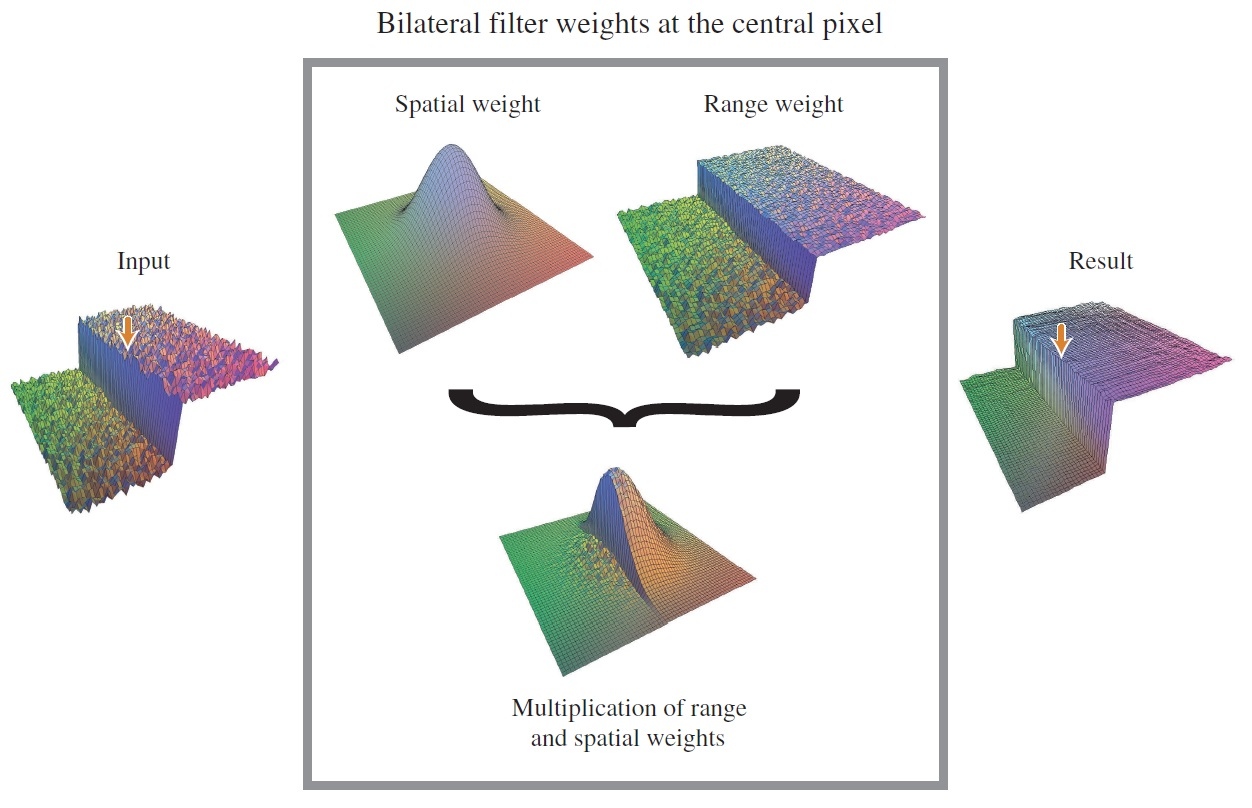
\includegraphics[width=0.85\linewidth]{bilateral_filter.jpg}}
	\caption{Bilateral filter for smoothing an input image \cite{Paris2008} }
	\label{fig:bilateral_filter}
\end{figure}

The improvement in bilateral filter can clearly been seen when we compare the results in Fig. \ref{fig:bilateral_filter} which are got from applying bilateral filter and Gaussian filter \cite{Gonzalez06DIP, Motwani2004}.

Bilateral filter is extremely easy to adapt. For color image, we can change the intensity difference to color difference in Eq.\ref{eq: eq1_bf} to get the desire output as below:

\begin{equation}\label{eq: eq1_bf_color}
BF\left [ I \right ]_{p}\,\buildrel \Delta \over = \,\frac{1}{w_{p}}\sum_{q \in S}{G_{\sigma _{S}}\left (\left || p-q \right || \right ) G_{\sigma_{r}}}\left ( \left | C_{p}-C_{q} \right | \right )C_{q}
\end{equation} 

Though bilateral may not be the best noise reducing filter but it is good and simple. Also, it can be used for tone mapping, relighting and texture editing. However, the nonlinear operator is hard to compute since it is complex and spatially varying kernels. Besides, it causes staircase effect, gradient reversal, and artifact near edges.

\begin{figure*}[t]
	\centering
	\begin{subfigure}{0.6\textwidth}
		\centering
		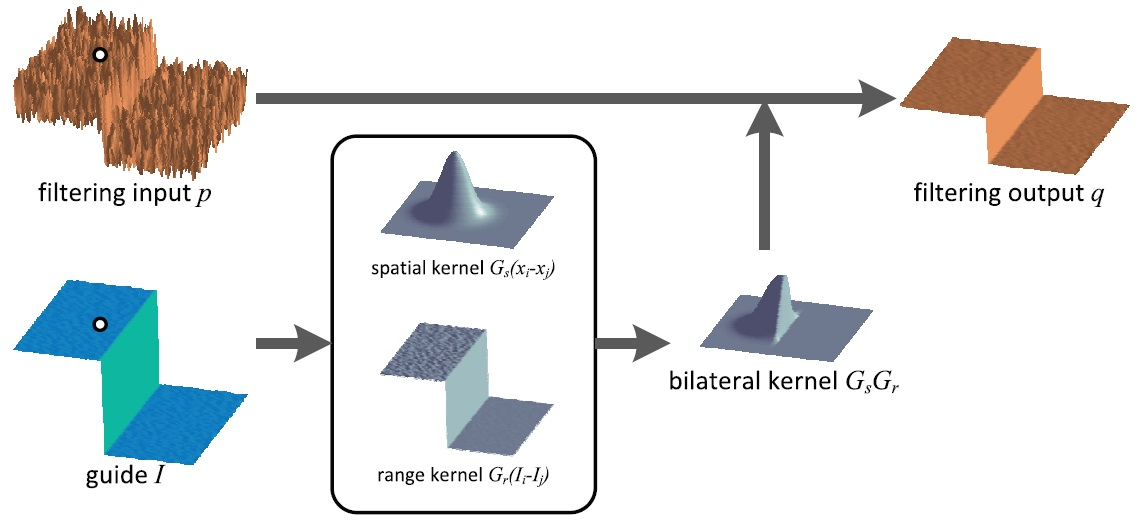
\includegraphics[width=0.95\linewidth]{bilateral_filter_process.jpg}
		\caption{}
		\label{fig:bilateral_filter_process}
	\end{subfigure}
	\begin{subfigure}{0.35\textwidth}
		\center{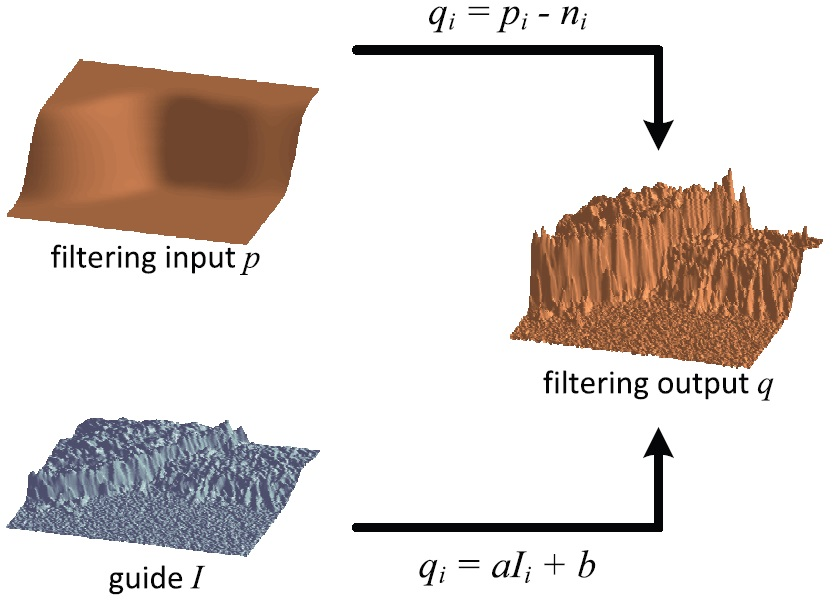
\includegraphics[width=0.95\linewidth]{guide_filter.jpg}}
		\caption{}
		\label{fig:guide_filter}
	\end{subfigure}%
	\caption{(a) Bilateral Filter Process and (b) Guided Filter Process }
	\label{fig:guide_bilateral_filter}
\end{figure*}

\begin{figure}[ht]
	\center{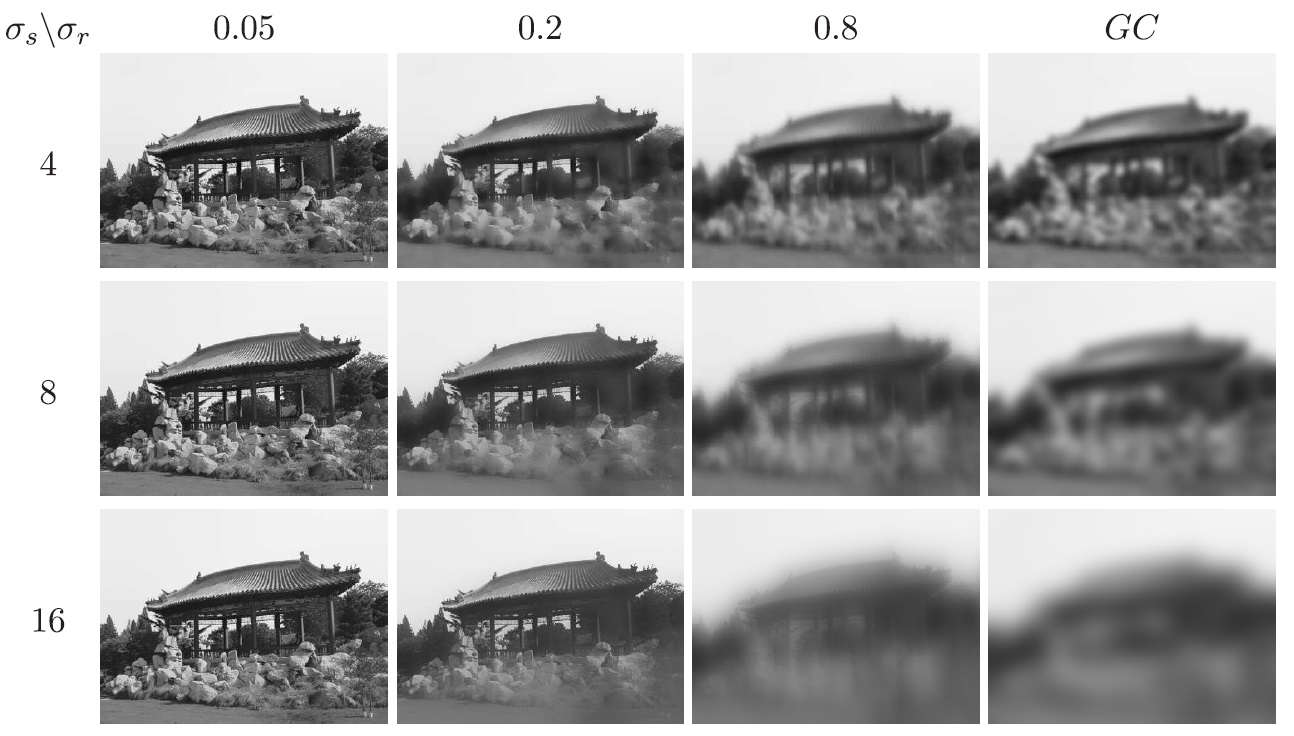
\includegraphics[width=1\linewidth]{bilateral_gauss.jpg}}
	\caption{Comparison between Bilateral and Gauss Filter with increasing spatial and intensity parameter  \cite{Paris2008} }
	\label{fig:bilateral_gauss}
\end{figure}

\subsubsection{Guided Image Filtering}
Guided image filter \cite{He2013} is an edge preserving smoothing filter, which output is locally a linear transform of the guidance image. It has good edge-preserving smoothing properties like bilateral filter but it solves the unwanted problems which occurs in bilateral filter.

The guided filtering process involves a guidance image $I$, a filtering input image $p$ and an output image $q$. Both $I$ and $p$ is given beforehand according to the application and they can be identical. Since we define that guided filter is a local linear model between the guidance image and the filtering output, we assume that $q$ is a linear transform of $I$ in a window $\omega_{k}$ centered at the pixel $k$ and is defined by:

\begin{equation}\label{eq: gif_01}
q_{i}=a_{k}I_{i}+b_{k},\forall i\in \omega_{k}, where 
\left\{\begin{matrix}
a_{k}=\frac{\frac{1}{\left |\omega\right |}\sum_{i\in \omega_{k}}{I_{i}p_{i}-\mu _{k}\bar{p}_{k}}}{\sigma_{k}^2+\epsilon}
\\ 
b_{k}=\bar{p}-a_{k}\mu_{k}
\end{matrix}\right.
\end{equation}

In Eq. \ref{eq: gif_01}, $\mu_{k}$ and $\sigma_{k}^2$ are the mean and variance of $I$ in $\omega_{k}$, $\left |  \omega \right|$ is the number of pixels in $\omega_{k}$ and $\bar{p}_{k}$ is the mean of $p$ in $\omega_{k}$.

We can also model the output $q$ as the input $p$ subtracting unwanted components $n$ as follows: 

\begin{equation}
q_{i}=p_{i}-n_{i}
\end{equation}

There are two cases in an input filter that should be consider which are "high variance" region and "flat patch". The idea of guided filter is that it determine "what is an edge that should be preserved"; hence, guided filter keep the high variance patch while the flat patch is smoothed which results in its good edge-preserving property.  Not only guided filter can preserve edges, it can also preserve gradient and transfer structure. Guided image filter can be fast implemented with the following Alg. \ref{alg:gif}.


\begin{algorithm}[htp]
	\caption {Guided Image Filtering}
	% \Titleofalgo { GuidedImageFiltering}
	
	\label{alg:gif}
	% \tcc{}
	\SetVline
	\KwIn{\\$p$: filtering input image.\\$I$: guidance image.\\$r$: radius.\\$\epsilon$: regularization.}
	\KwOut{\\$q$: filtering output image.}
	\linesnumbered
	\Begin {
		$mean_{I}=f_{mean}\left( I \right)$
		
		$mean_{P}=f_{mean}\left( P \right)$
		
		$var_{I}=corr_{I}-mean_{I}.*mean_{I}$
		
		$cov_{I_{p}}=corr_{I_{p}}-mean_{I}.*mean_{p}$
		
		$a = cov_{I_{p}}/\left( var_{I}+\epsilon \right)$
		
		$b=mean_{p}-a.*mean_{I}$
		
		$mean_{a}=f_{mean}\left( a \right)$
		
		$mean_{b}=f_{mean}\left( b \right)$
		
		$q=mean_{a}.*I+mean_{b}$
	}
\end{algorithm}

Note that $f_{mean}$ is the mean filter \cite{Gonzalez06DIP}, it can be replaced by Gaussian filter without having bad effect on performance of guided filter. 

\begin{figure}[ht]
	\center{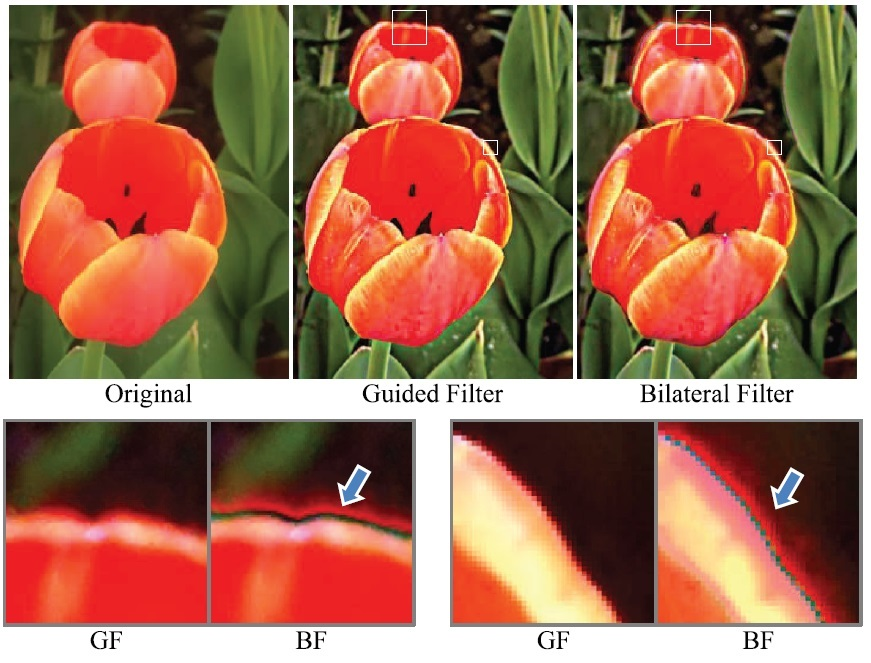
\includegraphics[width=0.7\linewidth]{guide_filter_result.jpg}}
	\caption{Detail enhancement comparing with Bilateral Filter with $r = 16, \epsilon = 0.1^{2}$ for Guided Filter , and $\sigma_{s} = 16, \sigma_{r} = 0.1$ for Bilateral Filter. \cite{He2013} }
	\label{fig:guide_filter_result}
\end{figure}

In the Fig. \ref{fig:guide_filter_result}, we can clearly see that guided image can avoid staircase effect and artifact that bilateral filter has. The result got from guided image is much better than the one got from bilateral filter.

\begin{figure}[ht]
	\center{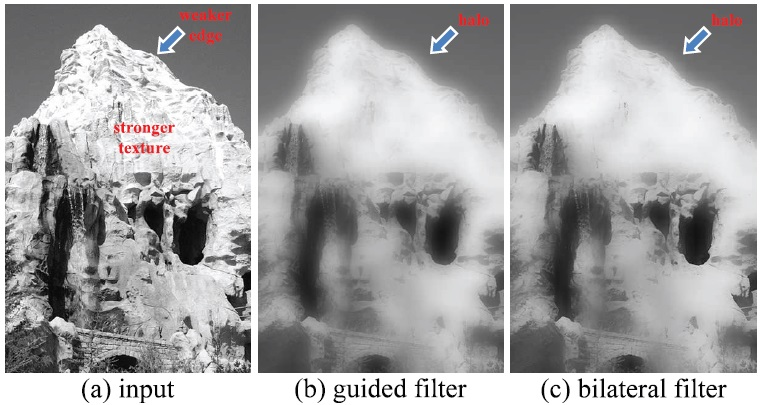
\includegraphics[width=0.7\linewidth]{guide_filter_result1.jpg}}
	\caption{The halo artifacts with $r = 16$, $\epsilon=0.4^{2}$ for  guided filter, $\sigma_{s}=16$, $\sigma_{r}= 0.4$ for bilateral filter.\cite{He2013} }
	\label{fig:guide_filter_result1}
\end{figure}
To sum up, guided filter has a $O(N)$ time non-approximate algorithm, independent of the window radius and the intensity range. Also, it is easily implement and avoid staircase effect and artifacts. It is good to be applied in feathering, matting, single image haze removal and joint up sampling. However, despite its advantage, guided filter also has its own limitation which is the exhibit halos near some edges when the image is being smoothing which is shown in Fig. \ref{fig:guide_filter_result1}.

\subsubsection{Non-linear variational methods with Total variational denoise}

The total variational method is first mentioned in the inverse problem when proposing regularizing criteria. It is based on the principle that signal has smooth details. So, denoise becomes the minimization problem, which finds a image in set of all images with bounded variation. It is applied effectively in noise reduction with smoothing image but preserving the edges.\cite{Rudin1992}\\
The original image can be approximated by ideal and noise image as

\begin{equation}
    \label{eq:tvl1_noise_model}
    f = u + n
\end{equation}
where $f$ is noisy image, $u$ is ideal image and $n$ is noise image which shows as Gaussian distribution with mean $0$.\\
Observing that $u$ has smooth in details, Rudin et. al \cite{Rudin1992} proposes the regularizing constraint for ensuing existing unique solution in an ill-posed problem for Eq.\ref{eq:tvl1_noise_model} as

\begin{equation}
    \label{eq:tvl1_denoise_rudin}
    \min_{u \in BV\left( \Omega \right)}\int_{\Omega}\left| \nabla u \left( x \right) \right|dx
\end{equation}
where first constraint assumes Gaussian Noisy with mean $0$ as\\

\begin{equation}
    \label{eq:tvl1_denoise_rudin_constraint_1}
    \int_{\Omega}u\left( x \right)dx = \int_{\Omega}f\left(x\right)dx
\end{equation}
and second constraint expresses noisy derivation $\sigma$ as\\

\begin{equation}
    \label{eq:tvl1_denoise_rudin_constraint_2}
    \int_{\Omega}\left| u \left( x \right) - f \left( x \right)\right|^{2}dx = \sigma^{2}\left|\Omega\right|
\end{equation}
In \cite{Chambolle2010}, Chambolle et. al changed Eq.\ref{eq:tvl1_denoise_rudin} into the following unconstrained minimization problem as

\begin{equation}
\label{eq:tvl1_denoise_rof}
\min_{u \in BV\left( \Omega \right)}\int_{\Omega}\left| \nabla u \right|dx + \frac{\lambda}{2}\left||u - f\right||_{2}^{2}dx
\end{equation}
where first term is the smoothness term, second term is data term to evaluate the accuracy of data and $\lambda$ is regularization constant.

Depend on normalization for the smoothness term, there are two model energy. First, ROF (Rudin, Osher and Fatemi) model uses $L_{1}$ normalization in the smoothness term as in Eq.\ref{eq:tvl1_denoise_rof}. Second, TV-L1 model uses $L_{2}$ normalization in data term as

\begin{equation}
\label{eq:tvl1_denoise_tvl1}
\min_{u \in BV\left( \Omega \right)}\int_{\Omega}\left| \nabla u \right|dx + \lambda\left||u\left( x \right) - f\right||dx
\end{equation}
TV-L1 and ROF models are the specific cases in general minimization energy problem\cite{Chambolle2010, Znah2013, Duran2013} , which defined as

\begin{equation}
    \label{eq:tvl1_denoise_general_min_energy}
    \min_{x}F\left(K_{x}\right) + G_{x}
\end{equation}
where $F$ and $G$ are functions satisfying convex property, and $K$ is linear operator. Clearly, data term and smoothness term in ROF and TV-L1 respectively express as

\begin{equation}
    \label{eq:tvl1_denoise_general_min_energy_smooth_rof}
    F\left(K_{x}\right) \deltaeq  \int\left|\nabla u\right|
\end{equation}

\begin{equation}
    \label{eq:tvl1_denoise_general_min_energy_smooth_rof}
    G_{ROF} \deltaeq  \int\frac{\lambda}{2}\left||x -f\right||^{2}
\end{equation}

\begin{equation}
    \label{eq:tvl1_denoise_general_min_energy_smooth_rof}
    G_{TV-L1} \deltaeq \int\lambda\left||x -f\right||
\end{equation}

Applying the Legendre-Fenchel transformation for $F$ with any $p \in X$, we obtain the dual formula $F^{*}$ of $F$ in Eq.\ref{eq:tvl1_denoise_general_min_energy} as

\begin{equation}
    \label{eq:tvl1_denoise_general_min_energy_dual}
    F^{*}\left(p\right) = \sup_{x \in X}\left<p, x\right> - F\left(X\right)
\end{equation}

Similarly, applying the transformation for $F^{*}$ where $F$ and $F^{*}$ are the convex function, we obtain the formula below:

\begin{equation}
    \label{eq:tvl1_denoise_general_min_energy_dual_dual}
    F = F^{**}\left(p\right) = \sup_{x \in X}\left<p, x\right> - F^{*}\left(X\right)
\end{equation}

Applying the above formula to $F$, we get the saddle formula as follows:

\begin{equation}
    \label{eq:tvl1_denoise_general_min_energy_saddle}
    \min_{x}\max_{p}  F\left(Kx, p\right) + G_{x} - F^{*}\left(p\right)
    \end{equation}
in which

\begin{equation}
    \label{eq:tvl1_denoise_general_min_energy_dual_ff}
    F^{*}\left(p\right) = \sigma_{P}\left(p\right) = \left\{\begin{matrix}
    0 & p \in P \\ 
    +\infty & p \notin P 
    \end{matrix}\right.
\end{equation}
where $P = \left\{ p: \forall_{i}\begin{Vmatrix}p_{i}\end{Vmatrix}\leq 1 \right\} $

In primal-dual algorithm, we define proximity operator which is equivalent to implicit gradient descent step, as below

\begin{equation}
    \label{eq:tvl1_denoise_general_proximity}
    \left(I + \tau \delta F\right)^{-1}\left(x\right)=arg\min_{x}\frac{1}{2}\begin{Vmatrix}y - x\end{Vmatrix}^{2} + \tau F\left(y\right)
\end{equation}

To implement Primal-Dual algorithm,$F^{*}$ and $G$ for ROF and TV-L1 are calculated as below

\begin{equation}
    \label{eq:tvl1_denoise_general_f_tilde}
    \left(I + \sigma \delta F^{*}\right)^{-1}\left(p\right) = \frac{p}{max\left(\begin{Vmatrix}p\end{Vmatrix}, 1 \right)}
\end{equation}

\begin{equation}
    \label{eq:tvl1_denoise_general_g_rof_tilde}
    \left(I + \tau \delta G_{ROF}\right)^{-1}\left(x\right) = \frac{x + \lambda \tau f}{1 + \lambda \tau}
\end{equation}

\begin{equation}
    \label{eq:tvl1_denoise_general_g_tvl1_tilde}
    \left(I + \tau \delta G_{TV-L1}\right)^{-1}\left(x\right) = \left\{\begin{matrix}
    x - \lambda \sigma & x > f +  \lambda \sigma\\
    x + \lambda \sigma & x < f -  \lambda \sigma\\
    f & \left|x - f\right|\leq \lambda \sigma\\
    \end{matrix}\right.
\end{equation}

\begin{algorithm}[ht]
	\caption {Primal Dual Algorithm}
	% \Titleofalgo {Dual Domain Image Denoise}
	\label{alg:primal_dual_general}
	% \tcc{}
	\SetVline
	\AlgoDisplayBlockMarkers\SetAlgoBlockMarkers{}{end}%
	\SetKwComment{tcc}{\%}{}
	\KwData
	{	
		\\
		+ Step size $\sigma > 0$, $\tau > 0$ \\
		+ $\sigma \tau L^{2} < 1$, where $L = \begin{Vmatrix}K\end{Vmatrix}$ \\
		+ $\theta = 1$\\
		+ X: Input
	}
	\Begin
	{
		$x_{i}$ = X\;
		$p_{i}$ = $\nabla x_{i}$\;
		\While{not convergence or not enough iteration}
		{
			$p_{i} = \left(I + \sigma \delta F^{*}\right)^{-1}\left(p_{i} + \sigma K x_{i}\right)$
			\tcc*[r]{Eq.\ref{eq:tvl1_denoise_general_f_tilde}}
			\BlankLine
			\tcc{Eq.\ref{eq:tvl1_denoise_general_g_rof_tilde} or \ref{eq:tvl1_denoise_general_g_tvl1_tilde}}
			
			$\hat{x}_{i} = \left(I + \tau \delta G\right)^{-1}\left(x_{i} - \tau K^{T} p_{i}\right)$\;
			\BlankLine
			$x_{i} = \hat{x}_{i} + \theta \left(\hat{x}_{i} - x_{i}\right) $\;
		}
	}	
\end{algorithm}

\subsection{Frequency Domain using Wavelet Shrinkage Denoising}
Wavelet shrinkage denoising \cite{fodor2003denoising} is considered a non-parametric method which attempts to remove noise and retain signal regardless of the frequency content of the signal. The basic idea behind this techniques is to use wavelets to transform the data into a different basis, where "large" coefficients correspond to the signal while "small" ones represent mostly noise. The wavelet coefficients are suitably modified and the denoised data is obtained by an inverse wavelet transform of the modified coefficients.

Let $\mathbf{Y}$, $\mathbf{X}$ and $\epsilon$ denote the observed data, the noiseless data and the error matrices respectively. The three main steps of denoising using the wavelet shrinkage technique are as follows:

\begin{itemize}
	\item Calculate the wavelet coefficient matrix $\mathbf{w}$ by applying a wavelet transform $\mathbf{W}$ to the data:

	\begin{equation}
	    \mathbf{w} = \mathbf{WY} = \mathbf{WX} + \mathbf{W\epsilon}
	\end{equation}
	
	\item Modify the detail coefficients to obtain the estimate $\mathbf{w}$ of the coefficients of $\mathbf{X}$:
	
	\begin{equation}
	    \mathbf{w} \rightarrow \hat{\mathbf{w}}
	\end{equation}
	
	\item Inverse transform the modified coefficients to obtain the denoised estimate:
	
	\begin{equation}
	    \hat{\mathbf{X}} = \mathbf{W}^{-1}\hat{\mathbf{w}}
	\end{equation}
\end{itemize}

\begin{figure}[ht]
	\center{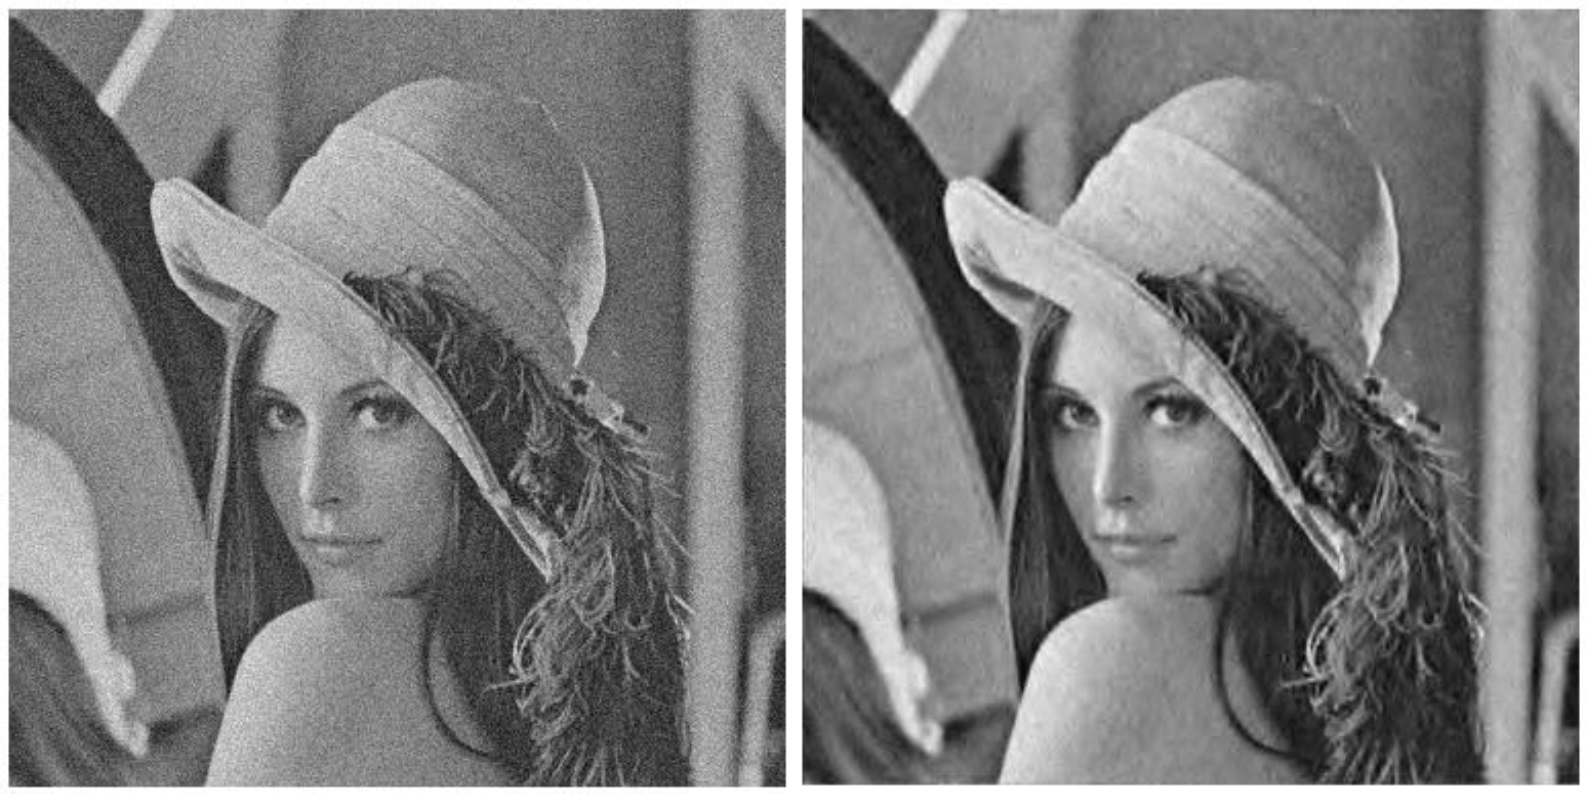
\includegraphics[width=1\linewidth]{wavelet_shrinkage.jpg}}
	\caption{(left) Noisy "Lena" image with $\epsilon = 20$ and (right) result output provided by Wavelet Shrinkage \cite{fodor2003denoising}}
	\label{fig:wavelet_shrinkage}
\end{figure}

Observing Fig. \ref{fig:wavelet_shrinkage}, it notes that the noise is removed yet the detail of the image is not smooth compared to other spatial filters. However, the color contrast is not consistent as well as the computation complexity is high. Also, in some cases, wavelet shrinkage create noticeable artifact that can considerably degrade the image.

\subsection{Integrated Spatial and Frequency Domain}
\subsubsection{Dual domain image denoising}
Dual domain image denoising (DDID) \cite{Knaus2013} is an iterative denoising method which combines both spatial and transform domains. Since each domain has its advantages and shortcomings, this combination complements and solves the problems that effects on the result output.  

Before DDID, there are several state-of-art approaches which combine both domain such as BM3D \cite{Dabov2008}, shape-adaptive BM3D (SA-BM3D) \cite{Dabov2008_1} and BM3D with shape-adaptive principal component analysis (BM3D-SAPCA) \cite{Dabov2009}. They denoise based on block-matching which introduces visible artifacts in homogeneous regions, expressing as low-frequency noise. Also, they are sophisticated which pay for the high quality with implementation complexity \cite{Lebrun2012}.   

DDID offers a simpler way to implement yet competes BM3D in quality. It combines two popular filters for two domains. For the spatial domain, the bilateral filter is used to preserve features like edges; however, it has difficulties preserving low contrast details. For the transform domain, short time Fourier transform \cite{Allen1977} with wallet shrinkage \cite{Donoho1995, Zong1996, Taswell2000, fodor2003denoising} is applied to preserve good detail though it suffers from ringing artifacts near steep edges.

\begin{figure}[ht]
	\center{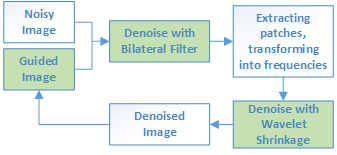
\includegraphics[width=1\linewidth]{ddid_process.png}}
	\caption{Dual Domain Image Denoising process}
	\label{fig:ddid_process}
\end{figure}

Given a noise-contaminated image $y = x + \eta$ with a stationary variance $\sigma^2=Var[\eta]$, the goal of DIDD is to estimate the original image $x$. The image is separated into two layers which are denoised separately. The high-contrast layer is bilateral filtered and the low-contrast layer is denoised using wavelet shrinkage. Thus, the original image can be approximated by the sum of two denoised layers as

\begin{equation}
\label{eq:did_ss}
\tilde{x} = \tilde{s} + \tilde{S},
\end{equation}

where $\tilde{s}$ and $\tilde{S}$ are the denoised high-contrast and low-contrast images.

In the first step, the denoised high-contrast values $\tilde{s}_{p}$ for a pixel $p$ is computed using a joint bilateral filter \cite{Paris2008}. The joint bilateral uses the guide image $g$ to filter the noisy image $y$. The bilateral kernel is defined over a square neighborhood window $\mathbf{\mathscr{N}}_{p}$ centered on every pixel $p$ with window radius $r$. The parameter $\sigma_{s}$ and $\gamma_{r}$ shape the spatial and range kernels respectively. The two denoised image high-contrast images is obtain as following:

\begin{equation}
\label{eq:did_gp}
\tilde{g}_{p}=\frac{\sum_{q\in \mathscr{N}_{p}}{k_{p,q}g_{q}}}{\sum_{q\in \mathscr{N}_{p}}{k_{p,q}}}
\end{equation}

\begin{equation}
\label{eq:did_sp}
\tilde{s}_{p}=\frac{\sum_{q\in \mathscr{N}_{p}}{k_{p,q}y_{q}}}{\sum_{q\in \mathscr{N}_{p}}{k_{p,q}}},
\end{equation}

where the bilateral kernel is

\begin{equation}
\label{eq:did_kpq}
k_{p,q}=e^{-\frac{\left| p-q\right|^2}{2\sigma_{s}^2}}e^{-\frac{\left( g_{p}-g_{q}\right)^2}{\gamma_{r}\sigma_{s}^2}}
\end{equation}

In the second step, for the wavelet shrinkage in the transform domain, the low contrast signals are extracted by subtracting the bilaterally filtered values $\tilde{g}_{p}$ and $\tilde{s}_{p}$ from $g_{p}$ and $y_{p}$, followed by multiplication with the range kernel of Eq. \ref{eq:did_kpq}. Then, the STFT is performed to transition these low-contrast signals to the frequency domain. The resulting coefficients $G_{p,f}$, and $S_{p,f}$, are presented for frequencies $f$ in the frequency window $\mathscr{F}_{p}$ with the same size as $\mathscr{N}_{p}$.

\begin{equation}
\label{eq:did_gpf}
G_{p,f}=\sum_{q\in \mathscr{N}_{p}}{e^{-i2\pi\left( q-p \right).f/\left( 2r+1 \right)}k_{p,q}\left( g_{q}-\tilde{g}_{p}\right)}
\end{equation}

\begin{equation}
\label{eq:did_sspf}
S_{p,f}=\sum_{q\in \mathscr{N}_{p}}{e^{-i2\pi\left( q-p \right).f/\left( 2r+1 \right)}k_{p,q}\left( y_{q}-\tilde{s}_{p}\right)}
\end{equation}

Assuming that the bilateral kernel $k_{p,q}$  is noise-free, the variance $\sigma_{p,f}^2$ of the noisy Fourier coefficients is

\begin{equation}
\label{eq:did_spf}
\sigma_{p,f}^2=\sigma^2\sum_{q\in \mathscr{N}_{p}}{k_{p,q}^2}
\end{equation}

In the last step, shrinkage factors similar to the range kernel of the bilateral filter is used. For the wavelet shrinkage factor $K_{p,f}$, the signal needs keeping and the noise needs discarding:

\begin{equation}
\label{eq:did_kpf}
K_{p,f}=e^{-\frac{\gamma_{f}\sigma_{p,f}^2}{\left| G_{p,f} \right|^2}}
\end{equation}

Like the bilateral kernel $k_{p,q}$, the shrinkage factors $K_{p,f}$, are defined using the spectral guide $G_{p,f}$, and the wavelet shrinkage parameter $\gamma_{f}$ plays a similar role as the bilateral range parameter $\gamma_{r}$. And the low-contrast value is yielded as following:

\begin{equation}
    \label{eq:did_tspf}
    \tilde{S}_{p}=\frac{1}{\left| \mathscr{F}_{p} \right|}\sum_{f\in \mathscr{F}_{p}}{ K_{p,f}S_{p,f}}
\end{equation}

Dual domain image denoise can be fast implemented with the following Alg. \ref{alg:ddid}.

\begin{algorithm}[ht]
	\caption {Dual Domain Image Denoise}
	% \Titleofalgo {Dual Domain Image Denoise}
	\label{alg:ddid}
	% \tcc{}
	\SetVline
	\KwData
	{	
		\\
		+ Bilateral range $\gamma_{r} = \left\{ 100, 8.7, 0.7 \right\}$ \\
		+ Wavelet shrinkage $\gamma_{f} = \left\{ 4.0, 0.4, 0.8 \right\}$\\
		+ Window radius $r = 15$\\
		+ Bilateral filter spatial $\sigma_{s} = 7$\\
	}
	\SetKwProg{Fn}{function}{}{}% algorithm function
	\SetKwFor{For}{parfor}{}{fintq}%
	\AlgoDisplayBlockMarkers\SetAlgoBlockMarkers{}{end}%
	\SetKwComment{tcc}{\%}{}
	\SetAlgoNoEnd
	\Fn{x = DDID(y, sigma2)}{
		x = step(y, y, sigma2, 15, 7, 100, 4.0)\;
		x = step(x, y, sigma2, 15, 7, 8.7, 0.4)\;
		x = step(y, y, sigma2, 15, 7, 0.7, 0.8)\;
	}
	
	\Fn{xt = step(x, y, sigma2, r, sigma\_s, gamma\_r, gamma\_f)}{
		[dx dy] = meshgrid(-r:r)\;
		h = exp(-(dx.\textasciicircum{}2 + dy.\textasciicircum{}2) / (2 * sigma\_s.\textasciicircum{}2))\;
		xp = padarray(x, [r r], 'symmetric')\;
		yp = padarray(y, [r r], 'symmetric')\;
		xt = zeros(size(x))\;
		\BlankLine
		\For{p = 1:numel(x), [i j] = ind2sub(size(x), p);}
		{
			\BlankLine
			\small{\tcc{Spatial Domain: Bilateral Filter}}
			g = xp(i:i+2*r, j:j+2*r)\;
			y = yp(i:i+2*r, j:j+2*r)\;
			d = g - g(1+r, 1+r)\;
			k = exp(- d.\textasciicircum{}2 ./ (gamma\_r * sigma2)) .* h\small{\tcc*[r]{Eq.\ref{eq:did_kpq}}}
			gt = sum(sum(g .* k)) / sum(k(:))\small{\tcc*[r]{Eq.\ref{eq:did_gp}}}
			st = sum(sum(y .* k)) / sum(k(:))\small{\tcc*[r]{Eq.\ref{eq:did_sp}}}
			\BlankLine
			\small{\tcc{Fourier Domain: Wavelet Shrinkage}}
			V = sigma2.* sum(k(:).\textasciicircum{}2) \small{\tcc*[r]{Eq.\ref{eq:did_spf}}}
			G = fft2(ifftshift((g - gt) .* k))
			\small{\tcc*[r]{Eq.\ref{eq:did_gpf}}}
			S = fft2(ifftshift((y - st) .* k))
			\small{\tcc*[r]{Eq.\ref{eq:did_sspf}}}
			K = exp(- gamma\_f * V ./ (G .* conj(G)))
			\small{\tcc*[r]{Eq.\ref{eq:did_kpf}}}
			St = sum(sum(S .* K)) / numel(K)
			\small{\tcc*[r]{Eq.\ref{eq:did_tspf}}}
			\BlankLine
			xt(p) = st + real(St)
			\small{\tcc*[r]{Eq.\ref{eq:did_ss}}}
		}
	}
	
\end{algorithm}

\subsubsection{Nonlocal dual denoising}
DDID provides better quality of denoised output as well as a simpler way to implement denoising method in both spatial and transform domains than any other state-of-art algorithms sharing the same idea. However, its processing time is slow and it also causes strong frequency domain artifacts unexpectedly. A later approach named Nonlocal Dual Denoising (NLDD) \cite{Pierazzo2014} has overcome those drawbacks. 

\begin{figure}[ht]
	\center{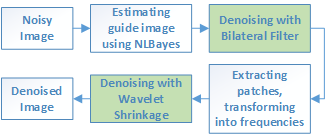
\includegraphics[width=1\linewidth]{nldd_process.png}}
	\caption{Non-local dual denoising process}
	\label{fig:nldd_process}
\end{figure}

The strong frequency domain artifacts are caused by the guide which is provided from the first two iterations of DDID algorithm. Since the DDID procedure is applied three times with different parameters, each time the result of the previous calculation is used as a guide. It notes that the image is denoised in the last iteration only and the other two are only used to obtain a suitable guide. Also, because of using the noisy image to be the guide in the first iteration and the kernel in Eq. \ref{eq:did_kpq} is computed from it, "parasite" information is reserved and transmitted in the following iterations. This yields a result that contains artifacts. Thus, NLDD chooses to use the guide image which is provided by NL-Bayes \cite{Lebrun2012} because it has less artifacts than the one computed in the first two iteration of DDID.

\begin{figure}[ht]
	\center{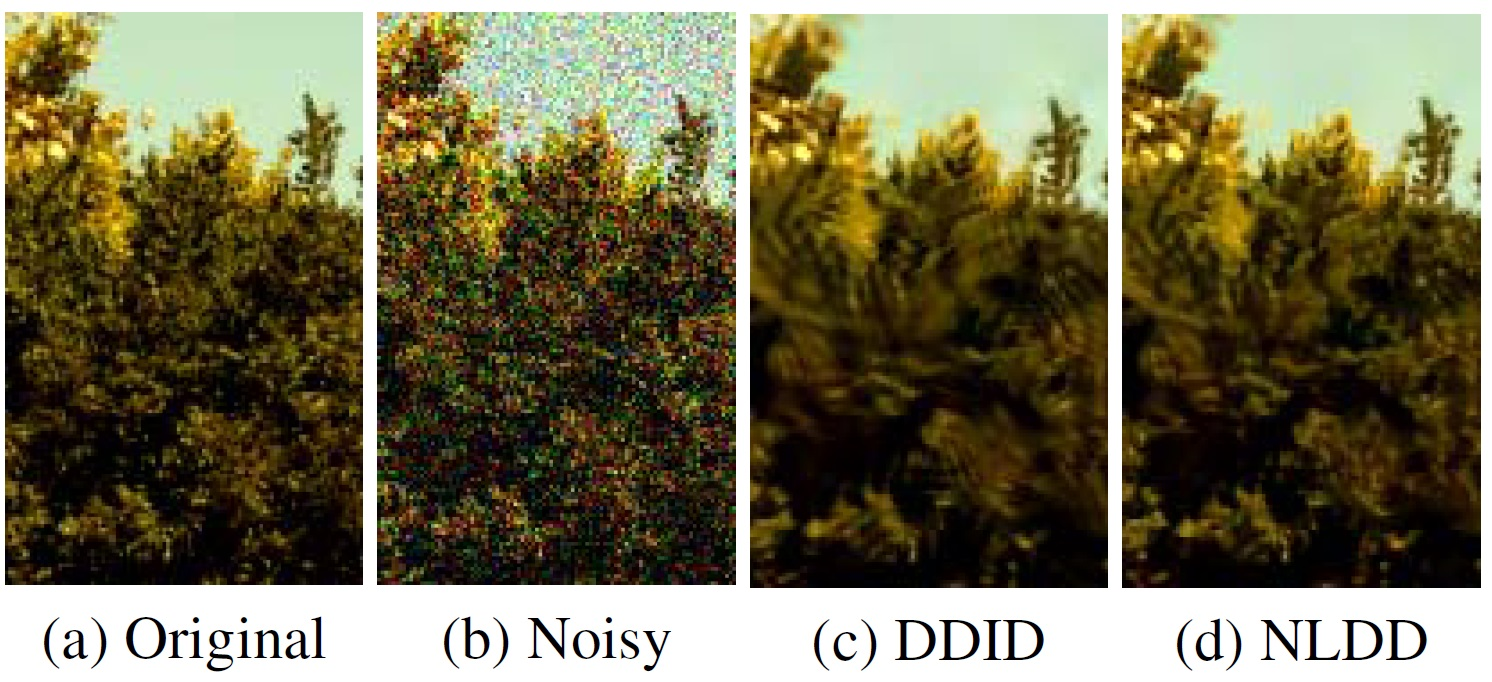
\includegraphics[width=1\linewidth]{nldd_result.jpg}}
	\caption{A detail of the artifacts produced by DDID and the corresponding result of NLDD. In this example $\sigma = 30$. \cite{Pierazzo2014} }
	\label{fig:nldd_result}
\end{figure}

Observing closely Fig. \ref{fig:nldd_result}, it notes that the ringing artifacts in denoised image of DDID does not present in result of NLDD. Besides, the processing time of NLDD algorithm has reduced 3 times because of the reduction of iterations which occurs in DDID.

%--------------------------------------------
%    Experiments and Discussions
%--------------------------------------------
\section{Experiments and Discussions}
\subsection{Evaluation Measures}
MSE (Mean-Square Error) is  the average of the squares of the errors about difference between original image and restored image

\begin{equation}
    \label{eq:mse}
    MSE = \frac{1}{mn}\sum_{i=0}^{m-1}\sum_{j=0}^{n-1}\left[I\left(i, j\right) - K\left(i, j\right)\right]^{2}
\end{equation}
where $I$ and $K$ respectively are the original image and restored image with size $m \times n$.

RMSE (Root-mean-square error) is dervied from MSE as below

\begin{equation}
    \label{eq:rmse}
    RMSE = \sqrt{MSE}
\end{equation}

PSNR (Peak Signal to Noise Ratio) is a term used to calculate the ratio between the maximum energy value of a signal and the noise energy influences the accuracy of the information. Because there are many wide variation signals, the PSNR is usually represented by the dB unit. The bigger the PSNR is, the better the image is. The formula is used to calculate PSNR as below

\begin{equation}
    \label{eq:psnr}
    PSNR = 10log_{10}\left(\frac{MAX_{I}^{2}}{MSE}\right)
\end{equation}
where $MAX_{I}$ is the maximum value of the pixel on the image.

\subsection{Noise models}
In this paper, we refer to the image noise problem caused by failure from gauss.The origin of Gauss noise in digital images is usually due to the sensor's image acquisition process affected by poor lighting, high temperature or signal transmission. Gauss noise is a addition, statistics noise with normal distribution. The probability density function p of the Gaussian random variable z is given by the formula\cite{Gonzalez06DIP}:

\begin{equation}
    \label{eq:gauss_noise}
    p\left(z\right) = \frac{1}{\sqrt{2\pi\sigma}}e^{-\left(z-\mu\right)^{2}}/2\sigma^{2}
\end{equation}
where $z$ represents the grey level, $\mu$  the mean value and $\sigma$  the standard deviation.

% \begin{comment}
Salt-and-pepper noise is a form of impulse noise caused by sharp and sudden disturbances in the image signal. Noise image will sparsely occurs white and black pixels.  The probability density function p of the random variable z in salt-and-pepper noise is given by the formula\cite{Gonzalez06DIP}:

\begin{equation}
    \label{eq:salt_and_pepper}
    p\left(z\right) = \left\{\begin{matrix}
    P_{a} & \text{with probability } a\\
    P_{b} & \text{with probability } b\\
    0 & \text{otherwise}\\
    \end{matrix}\right. 
\end{equation}
where $a$ and $b$ are two positive numbers with $a+b<1$, $\left[ P_{a}, P_{b}\right]$ is pixel value domain.

% \end{comment}

\subsection{Experiments}

In paper, we implement benchmark for denoise methods introduced above. Bilateral method has code from OpenCV. Guided image filter implements from guide of author in \cite{He2013}. In Guided image filter, we use guide images from bilateral filter and original filter. With TV-L1, we implements from \cite{Znah2013}. Lastly, we use reports from \cite{Pierazzo2014} on homepage to take results of DDID and NLDD methods.

Table \ref{tbl:result1} shows comparison methods such bilateral filter, guided image filter using bilateral filter and original input for guided image:

\begin{table}[ht]
	\centering
	\caption{PSNR comparision among noise image, Bilateral filter, Guided image filter with guide image using Bilater and original image}
	\label{tbl:result1}
	\begin{tabular}{|l|c|c|c|c|}
		\hline
		& \cellcolor[HTML]{C0C0C0}\textbf{Noise} 
		& \cellcolor[HTML]{C0C0C0}\textbf{Bilateral } 
		& \cellcolor[HTML]{C0C0C0}\textbf{Bilateral Guide} 
		& \cellcolor[HTML]{C0C0C0}\textbf{Original Guide} \\ 		
		\hline
		Alley &11.6 &20.51 &20.94 &24.44 \\ \hline
		Computer &11.96 &20 &19.99 &24.36 \\ \hline
		Dice &11.67 &22.44 &24.51 &36.84 \\ \hline
		Flowers & 12.39 & 20.29 & 20.66 & 31.28 \\ \hline
		Girl &11.69 &22.8 &25.08 &30.3 \\ \hline
		Traffic &11.78 &19.83 &19.74 &23.35 \\ \hline
		Trees &11.82 &18.3 &17.63 &19.41 \\ \hline
	\end{tabular}
\end{table}

Table \ref{tbl:result2} shows results of remain methods:

\begin{table}[ht]
	\centering
	\caption{PSNR comparision among TV-L1, Dual-domain image denoise and non-local dual denoise method}
	\label{tbl:result2}
	\begin{tabular}{|l|c|c|c|}
		\hline
		& \cellcolor[HTML]{C0C0C0}\textbf{TVL1} 
		& \cellcolor[HTML]{C0C0C0}\textbf{DDID} 
		& \cellcolor[HTML]{C0C0C0}\textbf{NLDD} \\
		\hline
		Alley &22.16 &25.3 &25.23 \\ \hline
		Computer &21.67 &25.95 &25.91 \\ \hline
		Dice &25.66 &32.33 &33.54 \\ \hline
		Flowers &21.84 &28.81 &29.46 \\ \hline
		Girl &26.47 &32.11 &32.94 \\ \hline
		Traffic &21.41 &24.63 &24.77 \\ \hline
		Trees &18.25 &20.25 &20.46 \\ \hline
	\end{tabular}
\end{table}

\begin{figure}[ht]
	\center{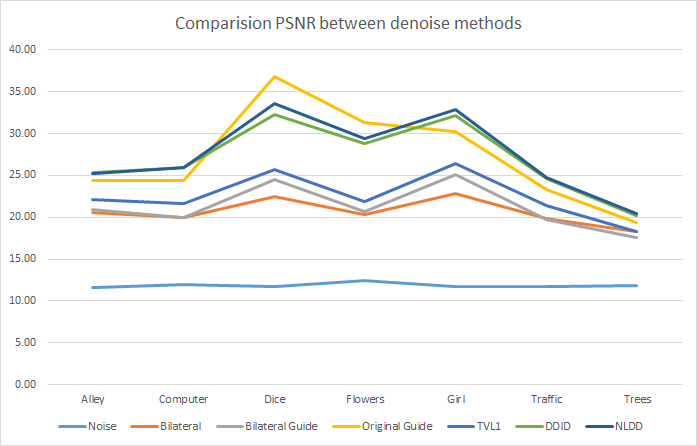
\includegraphics[width=1\linewidth]{psnr_methods.png}}
	\caption{Comparision PSNR between denoise methods}
	\label{fig:psnr_method}
\end{figure}

From Table \ref{tbl:result1} and \ref{tbl:result2}, DDID and NLDD methods have results better than remain methods. They take advantages of spatial and transform domain in denoise. 
Besides, we also see that images with many details such as Trees image, Traffic image will take lower results for all methods as Fig.\ref{fig:psnr_method}.

\begin{figure*}[ht]
	\centering
	\begin{subfigure}{0.5\textwidth}
		\center{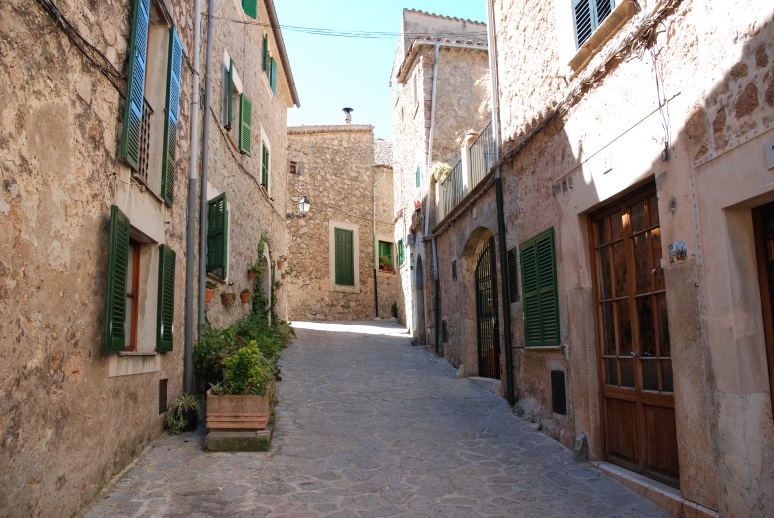
\includegraphics[width=0.95\linewidth]{data/Alley.jpg}}
		\caption{Original Image}
		\label{fig:Alley}
	\end{subfigure}%	
	\begin{subfigure}{0.5\textwidth}
		\center{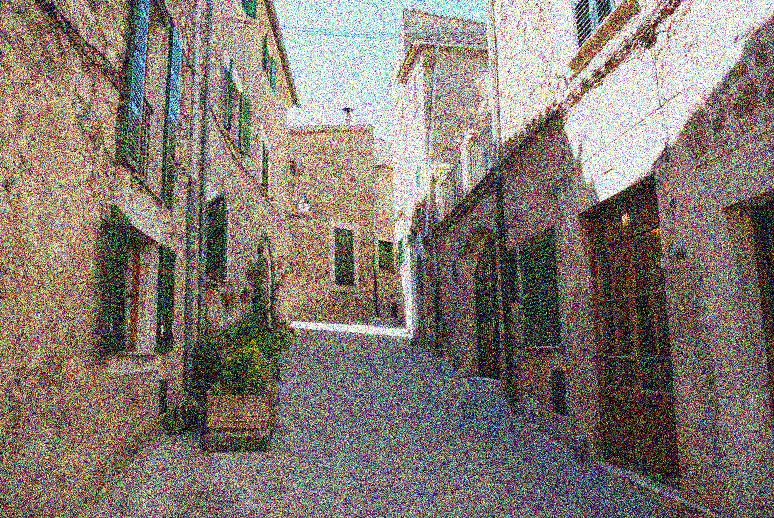
\includegraphics[width=0.95\linewidth]{data/Alley_80_noisy.jpg}}
		\caption{Gauss noisy images with $\sigma = 80$}
		\label{fig:NoisyAlley}
	\end{subfigure}	
	\begin{subfigure}{0.5\textwidth}
		\center{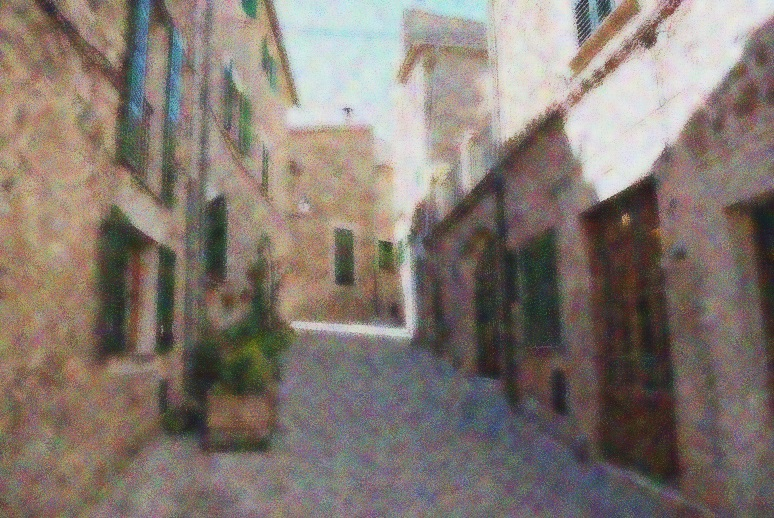
\includegraphics[width=0.95\linewidth]{data/Alley_80_Bilateral.jpg}}
		\caption{Bilateral with PSNR = 20.508}
		\label{fig:Alley_80_Bilateral}
	\end{subfigure}%
	\begin{subfigure}{0.5\textwidth}
		\center{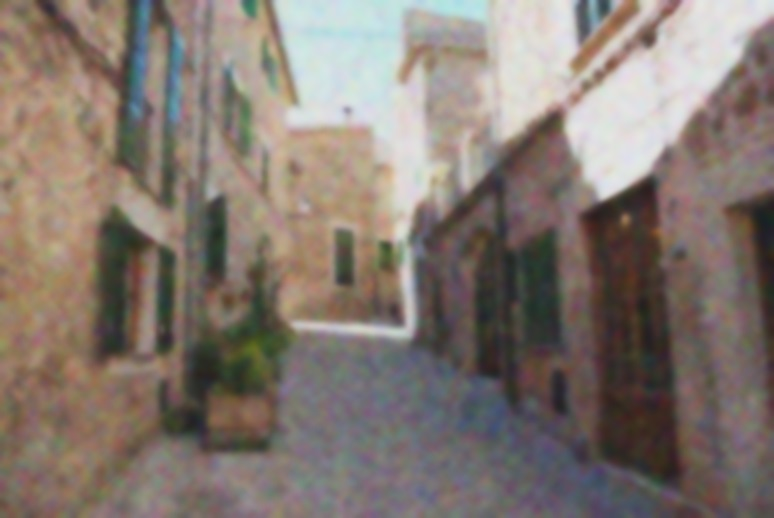
\includegraphics[width=0.95\linewidth]{data/Alley_80_BilateralGuided.jpg}}
		\caption{Bilateral Guided Image Filter with PSNR = 20.94}
		\label{fig:Alley_80_BilateralGuided}
	\end{subfigure}	
	\caption{Alley image with noise}
	\label{fig:alley_image}
\end{figure*}

\begin{figure*}[ht]
	\centering
	\begin{subfigure}{0.5\textwidth}
		\center{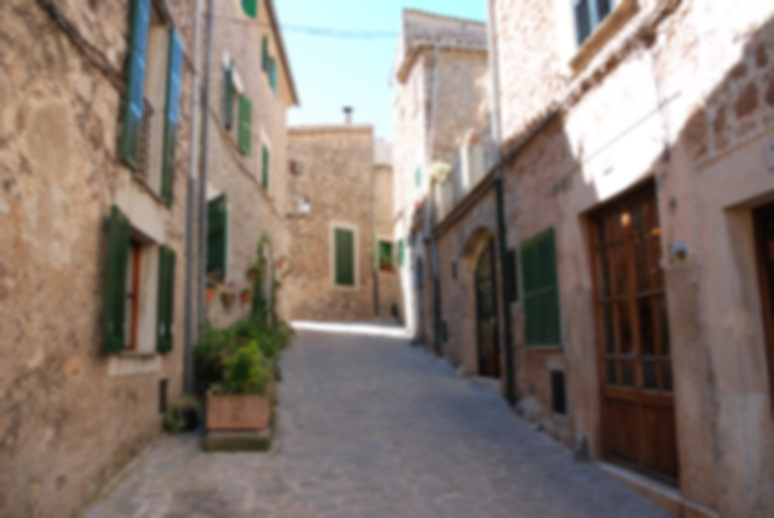
\includegraphics[width=0.95\linewidth]{data/Alley_80_OrginalGuided.jpg}}
		\caption{Original Guided Image Filter with PSNR = 24.44}
		\label{fig:NoisyFlowers}
	\end{subfigure}%
	\begin{subfigure}{0.5\textwidth}
		\center{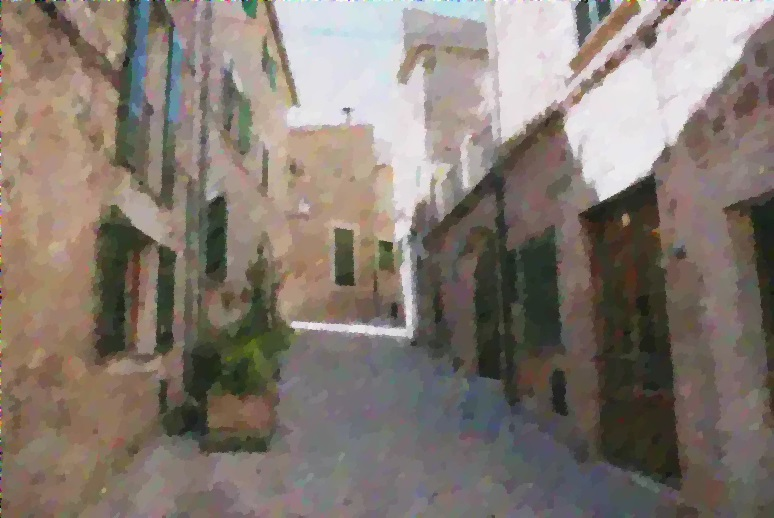
\includegraphics[width=0.95\linewidth]{data/Alley_80_TVL1.jpg}}
		\caption{TVL1 with PSNR = 22.16}
		\label{fig:Alley_80_TVL1}
	\end{subfigure}
	\begin{subfigure}{0.5\textwidth}
		\center{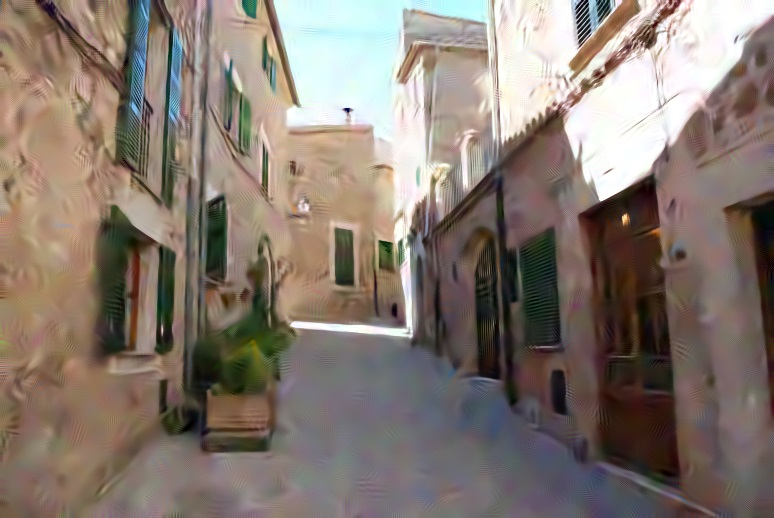
\includegraphics[width=0.95\linewidth]{data/Alley_80_DDID.jpg}}
		\caption{DDID with PSNR = 25.30}
		\label{fig:Alley_80_DDID}
	\end{subfigure}%
	\begin{subfigure}{0.5\textwidth}
		\center{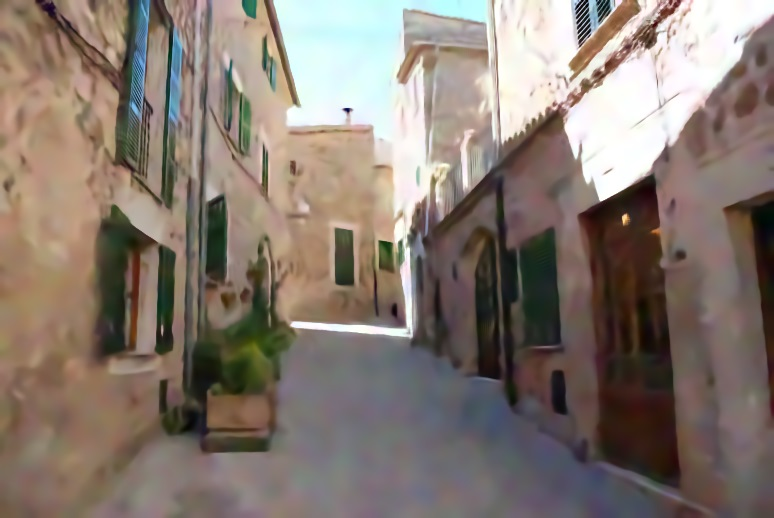
\includegraphics[width=0.95\linewidth]{data/Alley_80_DDID_nlb.jpg}}
		\caption{NLDD with PSNR = 25.23}
		\label{fig:Alley_80_DDID_nlb}
	\end{subfigure}
	\caption{Alley image denoise}
	\label{fig:Denoise Alley image}
\end{figure*}

%--------------------------------------------

%--------------------------------------------
%    Conclusions
%--------------------------------------------
\section{Conclusions}
To sum up, paper makes a survey for denoise methods. Bilateral filter, guided image filter and total variational methods process by spatial domain. In which, total variational method has good result more than remain methods. Besides, the results also shows NLDD, DDID are effective methods in denoise with not only hybrid approach but also spatial methods. From the survey, denoise also has many challenges when denoising on images too small details. 